\begin{wrapfigure}[12]{r}[0pt]{65mm}
	\caption{Circuito sommatore}
	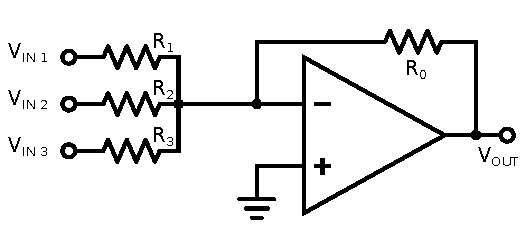
\includegraphics[width=65mm]{ccsum.pdf}
	\label{fig:ccsum}
\end{wrapfigure}

\section{Sommatore}

Il circuito riportato in Fig.(\ref{fig:ccinv}) è lo schema di un sommatore.
Tale circuito permette la somma di più segnali in input e risulta particolarmente comodo nel caso, ad esempio, della necessità di trasformare un numero digitale (bit) in numero analogico.
Analizziamo il circuito sempre assumendo un op-amp ideale.
Anche in questo caso $V_A$ sarà un ground virtuale.
Possiamo dunque imporre la seguente condizione: $\frac{V_1}{R_1}+\frac{V_2}{R_2}+\frac{V_3}{R_3}=\frac{-V_{out}}{R_0}$.
Dunque, se $R_0=R_1=R_2=R_3$ segue immediamtamente che $V_{out}=V_1+V_2+V_3$.
Ne abbiamo verificato il funzionamento utilizzando diversi segnali in input (tra cui onde quadre, segnali DC, cardiodi (???), ecc.).
Nelle seguenti figure sono riportati i segnali visualizzati a schermo sull'oscilloscopio.

$$grafici$$

Come vediamo il circuito si comporta da sommatore. I valori di resistenza utilizzate sono stati $R_0=(10.01\pm0.02)\si{\kilo\ohm}$, $R_1=(9.95\pm0.01)\si{\kilo\ohm}$, $R_2=(10.02\pm 0.01)\si{\kilo\ohm}$ e $R_3=(9.97\pm0.01)\si{\kilo\ohm}$.